\definecolor{Gray}{gray}{0.85}
\definecolor{LightCyan}{rgb}{0.88,1,1}

\section{Interface entre SE-STAR et le contrôleur}

Un grande partie de ce stage a tourné autour de l'interaction des algorithmes d'apprentissage par renforcement et SE-STAR (cf \ref{globalViewProject}). Cette partie sera consacrée à l'explication de l'architecture mise en place autour de SE-STAR pour la connection du contrôleur et de SE-STAR.
L'architecture proposée est composée de la création d'une \gls{API} simple pour communiquer avec SE-STAR et d'une interface bas niveau pour intégrer l'\gls{API} haut niveau (réalisée par Alexandre  kazmierowski).

Nous discuterons des divers difficultés que nous avons rencontré, des limites de notre architecture et des améliorations possibles.


SE-STAR est à la base un logiciel de simulation interne à THALES. SE-STAR a été prévu pour permettre une communication via l'\gls{API} de SE-STAR néanmoins le contrôle d'un seul agent par apprentissage par renforcement. Pourtant, l'API n'a pas été pensé pour un pilotae d'un agent par renforcement.  .Le contrôle des agents dans SE-STAR se base sur des stimulis internes motivationnels qui peuvent être configurés en fonction du rôle que l'on souhaite donner à un agent. Nous ne rentrerais pas dans les détails du fonctionnement original qui est complexe et orthogonal à notre objectif. Notre but est justement de créer un contrôle automatique se basant sur des stimulis extrinsèques (donnés par l'environnement) reposant sur la théorie de l'apprentissage par renforcement profond.

SE-STAR est un logiciel complexe. Il a donc fallu créer une interface  avec le contrôleur en étant le moins intrusif possible sur le code source de SE-STAR. L'objectif était de produire un code réutilisable quelques soit l'environnement. Nous nous rendrons compte que ce choix implique une perte en performance.

\begin{figure}[!h]
\centering
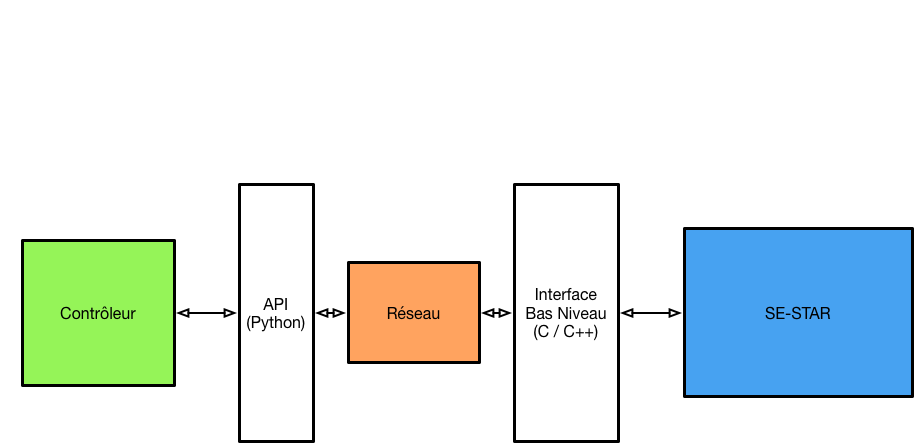
\includegraphics[width=.9\linewidth]{./assets/interfaceReseau/overviewInterface}
\caption{Vue globale de l'interaction entre le contrôleur et SE-STAR}
\end{figure}

\subsection{Analyse fonctionnelle de l'\gls{API} choisie}

Nous allons profiter de la simplicité de notre API pour l'expliquer. En apprentissage par renforcement,  un agent reçoit l'état dans lequel il se trouve. A partir de celui-ci, il interagit avec l'environnement qui lui répond en envoyant le prochain état et la récompense associée à l'état. Nous allons nous baser sur ce fonctionnement pour créer notre \gls{API}. 


\bigskip

% { --

\setlength{\arrayrulewidth}{.7mm}
\setlength{\tabcolsep}{12pt}
\renewcommand{\arraystretch}{2.}

\begin{center}
{\rowcolors{2}{white!80!gray!50}{gray!50!white!60}
\begin{tabular}{ |p{2cm}|p{8cm}|  }
\hline
\multicolumn{2}{|c|}{\gls{API} Client} \\
\hline
Fonction & Explication \\
\hline
Reset & Reset a pour but de redémarrer la simulation (obligatoire en cas de fin de partie ou si un certain temps est dépassé) \\
\hline
Step & \begin{enumerate}
\item Entrée: l'action effectuée
\item Sortie: une liste contenant l'état suivant, la récompense reçue, un booléen indiquant si la simulation est terminée et un dictionnaire donnant une multitude d'informations sur la simulation.
\end{enumerate} \\
\hline
Connect & Une fonction nous permettant d'établir une connection à distance avec un Windows distant. Nous ne parlerons pas de la méthode de connection à distance qui est assez complexe et reposant sur des outils tiers (Winexe, ...) \\
\hline
\end{tabular}
}
\end{center}

% -- May need change if set.. are not local }


L'\gls{API} est simple mais correspond exactement à la boucle classique en renforcement. Alexandre Kazmierowski a construit le serveur répondant à ces appels. L'outil créé par M. Kazmierowski permet l'interconnexion entre SE-STAR et le client .

\subsection{Principales limites et contraintes}

La simulation SE-STAR fonctionne actuellement uniquement sur Windows. Cela pose un problème car les différents outils, pour créer des algorithmes de Deep Learning, utilisent une distribution linux. Les échanges réseaux entre Linux et Windows limitent drastiquement le nombre d'images par seconde que peut recevoir l'agent (définissant la vitesse de simulation) car l'envoi d'un tableau de pixels sur le réseau est intrinsèquement coûteux. 

De plus, nous avons été confronté à de nombreux problèmes de déconnections impromptues qui ont nécessité la mise en place de mécanismes de reconnections automatiques. Néanmoins l'architecture mise en place manque encore de stabilité et n'est pas robuste à tous les types d'erreurs pouvant être rencontrés.

L'algorithme utilisé pour contrôler l'agent dans SE-STAR a été l'\gls{A3C} qui repose sur de multiples agents qui jouent dans l'environnement de façon asynchrone. Cela multiplie le nombre d'appels réseau et joue sur la stabilité de celui-ci, cela accroît la latence des appels agent (SE-STAR) / algorithme (Contrôle). De façon empirique, nous nous apercevons qu'il y a des problèmes dès que le nombre d'agents est supérieur à six. Cela s'explique en partie par le fait que SE-STAR est un logiciel demandant beaucoup de ressources, Or celui-ci n'a jamais été prévu pour une utilisation demandant de faibles ressources.Ainsi la multiplication des instances de SE-STAR peut causer des problèmes sur la machine cotée serveur si elle n'a pas assez de puissance. Alexandre  Kazmierowski nous a permis d'alléger les ressources demandées, permettant d'augmenter le nombre d'agents.

Nous pouvons dès lors nous demander si la stratégie asynchrone d'entraînement est viable.
Une problématique inhérente aux algorithmes de renforcement, qui découle de l'utilisation du deep learning, est le besoin de décorréler les états lors de l'entraînement . Or dans le cadre de nos algorithmes, cela s'avère difficile. La stratégie d'entraînement asynchrone permet la décorrélation des états lors de l'apprentissage.


En ajoutant les défaults de l'A3C, nous pouvons nous demander si d'autres algorithmes ne seraient pas plus pertinents.

\subsection{Compromis et solutions envisagées}

Dans cette partie, nous allons expliquer les solutions envisagées pour éviter de surcharger le réseau. Avant cela, il convient de revenir sur certaines contraintes sur le contrôle. En particulier, nous souhaitions avoir un contrôle qui est le moins intrusif possible sur l'environnement en l'occurrence SE-STAR.

Nous allons cependant proposer une méthode qui reste intrusive mais permet de résoudre en partie les problèmes liés à la multiplication des instances de SE-STAR et de réduire les appels réseaux. 

La méthode qui sera développée se nomme: Efficient Parallel Methods for Deep Reinforcement Learning \cite{2017arXiv170504862C}. Nous ne rentrerons pas dans les détails de l'algorithme car il est similaire à l'A3C \cite{DBLP:journals/corr/MnihBMGLHSK16}. Néanmoins,il propose une approche synchrone permettant l'utilisation du GPU. L'idée de ce papier est de proposer une architecture synchrone permettant de décorréler les états utilisés pour l'entrainement. A chaque pas, le contrôleur va décider quelles actions vont effectuer un ensemble d'agents. Le contrôleur va récupérer l'ensemble des états et des récompenses pour l'apprentissage et le choix de la nouvelle action. Quand le contrôleur rentre en phase d'apprentissage, il a un ensemble de transitions (état précédant, état actuel, action, récompense) décorrélées (car venant d'agents différents). Les premiers essais sont encourageants mais l'apprentissage n'est pas assez stable.

\begin{figure}[h!]
\begin{center}
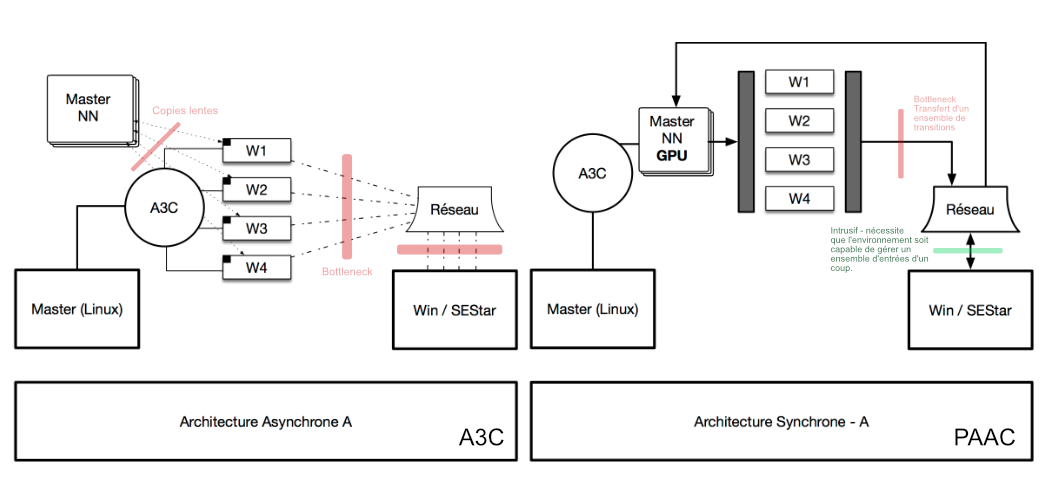
\includegraphics[scale=.4]{./assets/interfaceReseau/paaca3c}
\caption{Comparatif des algorithmes PAAC / A3C en mettant l'accent sur les problématiques réseaux}
\end{center}
\end{figure}

Nous remarquons que les principaux problèmes qui découlent de la stratégie asynchrone d'entrainement (A3C) sont liés à la communication réseau mais pas seulement. Un stratégie asynchrone exclue l'utilisation du \gls{GPU}. La stratégie synchrone de la \gls{PAAC} permet l'utilisation du GPU et impose que la simulation soit capable de gérér un ensemble d'actions en entrée. De plus, la question des transferts sur le réseau n'est pas résolue par cette approche. 

La véritable question est de savoir s'il n'existe pas d'autres approches qui suppriment la nécessité du réseau ou qui reposent sur des outils spécialement crées pour gérer les difficultés inhérentes aux réseaux. Nous verrons rapidement deux approches idéales se basant sur un outil Docker \cite{Merkel:2014:DLL:2600239.2600241} et sur l'utilisation de \gls{Wine} (qui permet de faire fonctionner des applications Windows sur Linux)

\subsection{Solutions idéales}

\subsubsection{SE-STAR sous linux via \gls{Wine}}
Notre objectif a été d'utiliser SE-STAR nativement sous Linux. Pour cela, il y a deux solutions. 
Premièrement, nous pouvons compiler directement SE-STAR pour Linux. Le problème est que le logiciel a été pensé pour une utilisation Windows et utilise des certaines librairies uniquement disponibles sur Windows. Nous ne savons pas si cela est possible même si cela aura le mérite d'être essayé. 
Deuxièmement, nous pouvons passer sous Wine pour utiliser une application Windows. Après une phase de configuration compliquée pour utiliser Wine, nous avons été en capacité d'utiliser SE-STAR sous Linux et d'utiliser l'\gls{A3C}. Nous avons remarqué des interruptions complètes de SE-STAR au bout d'une dizaine de minutes. Pour l'instant, il est difficile de savoir ce qui est responsable de ces interruptions. Nous pensons toujours que Wine est une solution viable. Il est reste néanmoins à comprendre l'origine des problèmes. Une des problématiques qui survient avec l'utilsation de Wine est que les fonctionnalités permises par SE-STAR ne sont pas entièremenet prise en charge par Wine. Cela nous oblige donc à passer par une version obsolète de Wine et possiblement moins stable.

\subsubsection{Une architecture scalable d'entrainement via Docker}
Nous allons présupposer que nous avons un moyen d'utiliser SE-STAR sous Linux. Nous exploiterons Docker (qui est un système de conteneurisation, qui groupe une application avec un environnement Linux léger configuré au préalable). Cela permet, en spécifiant les dépendances de SE-STAR, de pouvoir déployer dans un réseau n instances de SE-STAR et de simplement utilser le \emph{swarm mode} de docker pour avoir une gestion du réseau (load balancing, ...). Nous  pourrions imaginer déployer dans un cluster de cpu (ou gpu) plus de 1000 instances de SE-STAR gérées par le swarm mode de Docker. Ce genre d'architecture a déjà été utilisée.Cela pourra être mis en place dès que SE-STAR sera disponible sous Linux.

\begin{center}
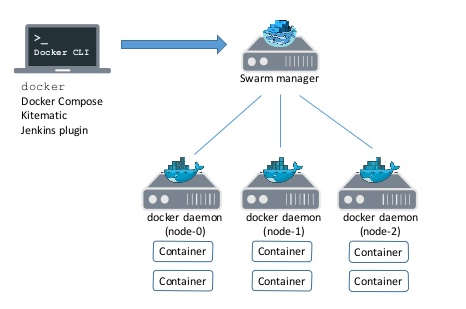
\includegraphics[scale=.5]{./assets/interfaceReseau/docker}
\captionof{figure}{Simple vue d'ensemble de l'utilisation de Docker en swarm mode}
\end{center}


Le swarm mode de Docker est une architecture composée d'un (ou plusieurs) noeud manageur qui a pour but de contrôler les noeuds enfants, de gérer le load balancing, la gestion des erreurs des noeuds enfants ... En ayant des conteneurs avec les dépendances requises par SE-STAR et l'application SE-STAR dans chaque conteneurs enfants, cela permet d'utiliser les algorithmes classiques d'apprentissage par renforcement profond à un échelle industrielle.

\subsection{Conclusion sur les questions d'interfaces et de réseaux}

A travers ce chapitre, j'ai essayé de vous expliquer les principaux enjeux dans le cadre de l'interface entre SE-STAR et les algorithmes d'apprentissage. Sur des cas jouets, ces problématiques ne font pas surfaces néanmoins, dans des applications industrielles nous sommes obligé de réfléchir à l'architecture dans laquelle nous allons déployer nos algorithmes et nos applications. Or, les \gls{frameworks} d'apprentissage et les applications peuvent être destinées à des environnements différents ou pire avoir des dépendances contradictoires. Il est donc essentiel  d'utiliser des applications capables d'isoler une application afin que celle-ci puisse être  disponible sur le réseau dans le but de pouvoir permettre la communication entre les applications.

Ci-dessous, un schéma récapitulatif de l'architecture idéal (qui a été partiellement mise en place durant le stage).


\begin{center}
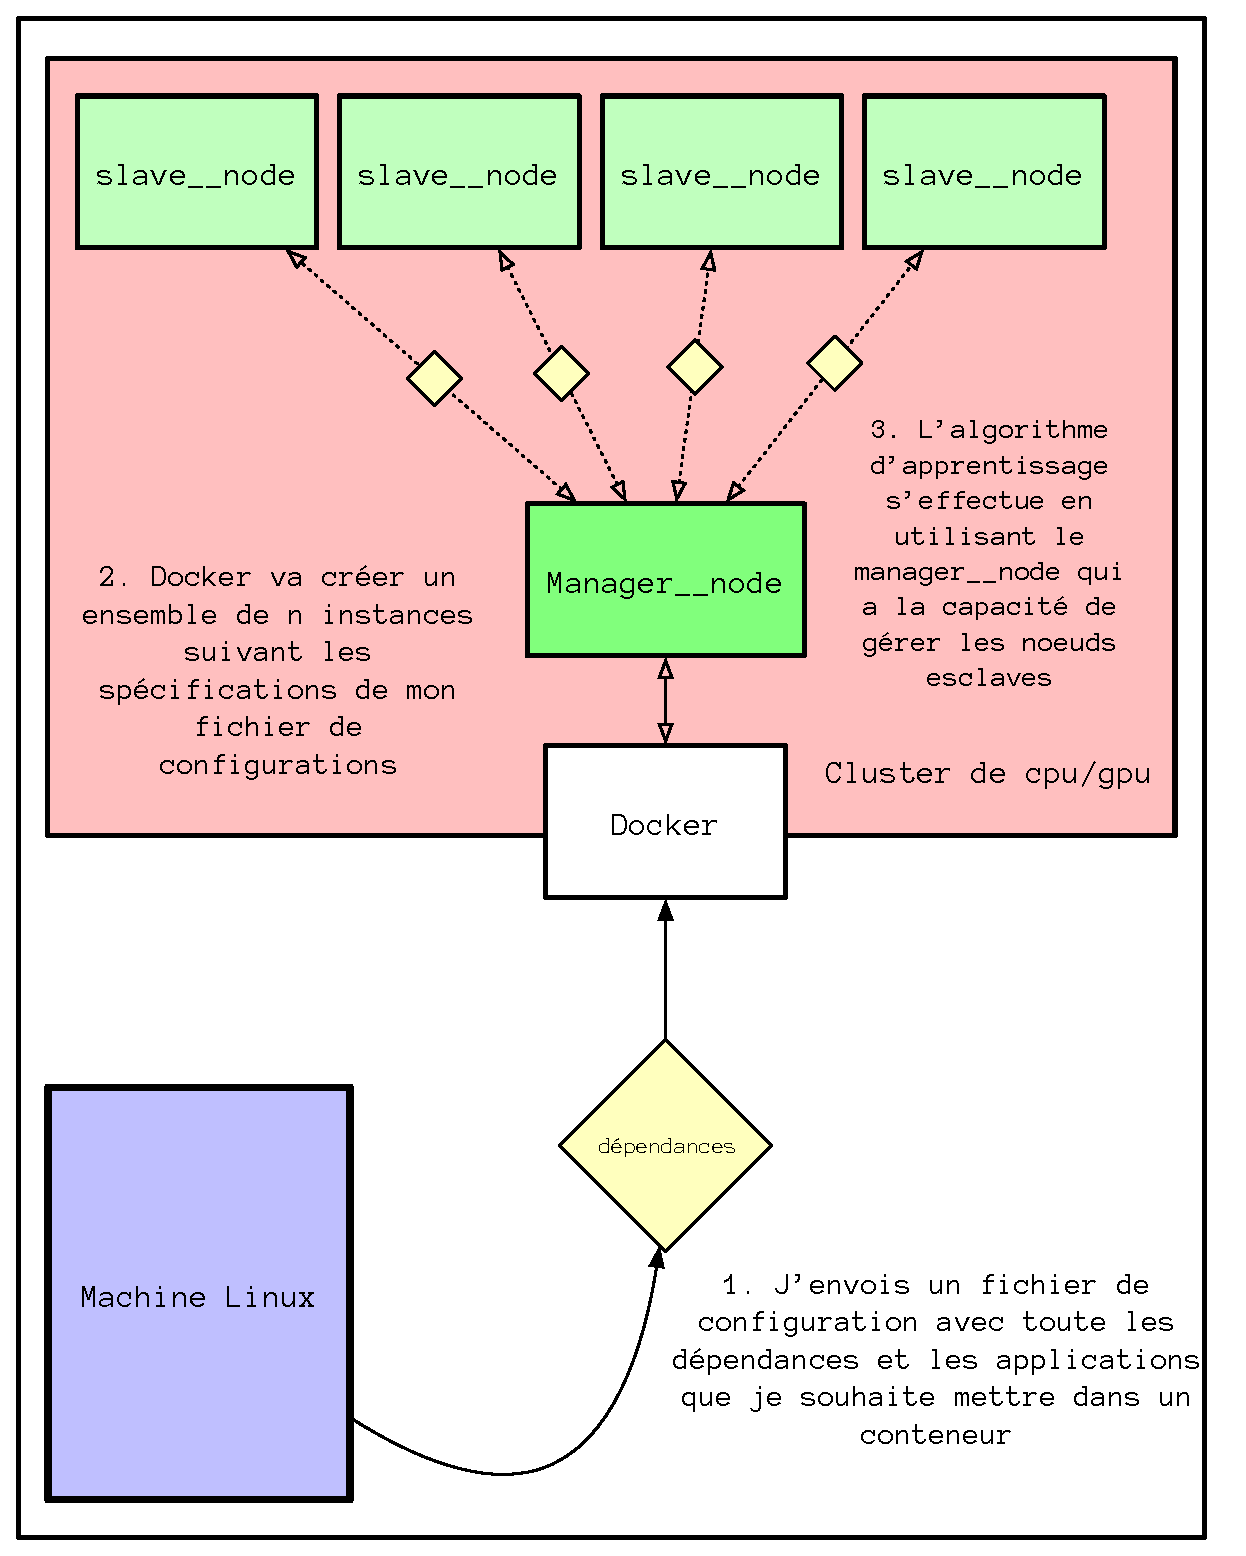
\includegraphics[scale=.7]{./assets/interfaceReseau/interfaceResume.eps}
\captionof{figure}{Vue d'ensemble de l'architecture partiellement mise en place dans le cadre de l'apprentissage de l'algorithme}
\end{center}
